\newpage

\paragraph{\LARGE Aufgabe 7 - Verzeichnisse}

\section{Aufgabenstellung}
	\subsection{Aufgabe 1: Typische Verzeichnisstrukturen}
		\begin{quote}
			\begin{itemize}
				\item Geben Sie die typische Verzeichnisstruktur einer aktuellen Linuxdistribution an. Was ist in den Verzeichnissen enthalten? Nennen Sie mindenstens f\"unf Beispiele (wie /etc, /usr usw.). Finden Sie zus\"atzlich heraus, wo Log-Dateien gespeichert werden. Wo liegen ausgelagerte Inhalte des Hauptspeichers?\\
				\item Geben Sie die typische Ordnerstruktur von Microsoft Windows an. Nennen Sie analog zur vor vorherigen Aufgabe einige beispielhafte Inhalte der jeweiligen Verzeichnisse (wie z.B, C:\textbackslash Windows\textbackslash System32).\\
			\end{itemize}
		\end{quote}
	\subsection{Aufgabe 2: Verzeichnisse}
		\begin{quote}
			Entwickeln Sie ein Programm myls, das den Inhalt von Verzeichnissen ausgibt. Die grundlegende Funktion ist in etwa vergleichbar mit dem Shell-Kommando ls.\\ \\
			Randbedingungen: \\
			\begin{itemize}
				\item Der Name des auszulesenden Verzeichnisses soll dem Programm als Argument \"ubergeben werden. Wird kein Verzeichnis angegeben, so wird das lokale Verzeichnis ausgegeben.\\
				\item Sie sollen die Funktionen opendir(), readdir() und closedir() verwenden, um die Eintr\"age des Verzeichnisses abzufragen.\\
				\item F\"ur den Zugriff auf Informationen zu den Eintr\"agen kann die Funktion lstat() verwendet werden. Diese lifert deterillierte Informationen zu jedem Verzeichniseintrag. Sie sollen mindestens die Attribute abragen und ausgeben, die bei Eingabe des Befehls ls -algo auf UNIX / Linux-System ausgegeben werden.\\
				\item Ihr Programm soll hinsichtlich der beiden Optionen -a und -l parametrisierbar sein die beiden Parameter k\"onnen auch zusammen angewendet werden, also myls -a -l oder myls -al. Hinsichtlich der Bedeutung der Parameter k\"onnen Sie sich an dem Standard-UNIX/Linux-Kommando orientieren.\\
				\item Verwenden Sie getopt(), um die Ausgabeparameter von der Kommandozeile einzulesen.\\
				\item Ihr Programm braucht keine weiteren Argumente oder Parameter zu unterst\"utzen.\\
				\item Geben Sie bei gesetzter Option -l den Namen ausf\"uhrbarer Dareien in rot und den Namen von C-Dateien (Dateiendung: .c) in gr\"un aus. Nutzen Sie f\"ur die Einf\"arbung von Verzeichniseintr\"agen Escape Sequenzen, die Sie beispielsweise unter http://www.linupedia.org/opensuse/Farbe\_in\_der\_Konsole finden.\\
			\end{itemize}
		\end{quote}
\newpage
\section{Aufgabe 7.1}
	\subsection{Vorbereitung}
		\begin{quote}
			Den Eintrag Verzeichsstuktur aus \\ ''https://wiki.ubuntuusers.de/Verzeichnisstruktur/'' lesen\\
		\end{quote}
	\subsection{Durchführung}
		\begin{quote}
			Ergebnisse recherchieren und protokollieren.\\
		\end{quote}
	\subsection{Fazit}
		\begin{quote}
			Aufgabe 7.1.1\\ \\
			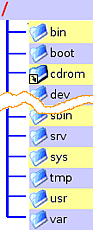
\includegraphics[width=2.0cm]{images/linux_verzeichnisstruktur}
			/bin:\\
			Enth\"alt f\"ur Linux unverzichtbare Programme.\\ \\
			/boot:\\
			Enth\"alt zum Booten benötigte Dateien.\\ \\
			/dev:\\
			Enth\"alt alle Gerätedateien, \"uber die die Hardware im Betrieb angesprochen wird.\\ \\
			/etc:\\
			Enth\"alt Konfigurations- und Informationsdateien des Basissystems.\\ \\
			/lib:\\
			Enth\"alt unverzichtbare Bibliotheken fürs Booten und die dynamisch gelinkten Programme des Basissystems.\\ \\
			/var/log:\\
			Enth\"alt alle Log-Dateien der Systemprogramme.\\ \\
			/var/cache ist vorgesehen als Datenpuffer für Anwendungsproramme.\\ \\ \\
			Aufgabe 7.1.2\\ \\
			C:\textbackslash Users:\\
			Enth\"alt Verzeichnisse der Benutzer.\\ \\
			C:\textbackslash Files:\\
			Enth\"alt  installierte Programme.\\ \\
			C:\textbackslash Temp:\\
			Enth\"alt  tempor\"are Dateien.\\ \\
			C:\textbackslash Windows\textbackslash Help:\\
			Enth\"alt  Hilfe-Dateien.\\ \\
			C:\textbackslash Windows\textbackslash Fonts:\\
			Enth\"alt  Schrifttyp-Dateien\\ \\
			C:\textbackslash Windows\textbackslash Logs:\\
			Enth\"alt alle Log-Dateien der Systemprogramme.\\ \\
			C:\textbackslash pagefile.sys:\\
			Speichert ausgelagerte Inhalte des Hauptspeichers.\\ \\
		\end{quote}

\section{Aufgabe 7.2}
	\subsection{Vorbereitung}
		\begin{quote}
			C-Projekt anlegen.\\
			Makefile schreiben.\\
		\end{quote}
	\subsection{Durchführung}
		\begin{quote}
			Code schreiben und dann testen bzw debuggen.\\
		\end{quote}
	\subsection{Fazit}
		\begin{quote}
			Randbedingung 1:\\ \\
			\tiny\lstinputlisting[language=C, firstline=21, lastline=53]{../src/myls.c}
			In der Variable ''argv'' sind  die Kommandozeilenparameter die \"ubergeben sind gespeichert. Dann wird mit ''getopt'' die Flags abgearbeitet. In der Variable ''optind'' (Zeile 48) ist der Index f\"ur das Element nach dem letzten Flag gespeichert.  Ist der index kleiner als die in ''argc'' \"ubergebene Anzahl dann wird das entsprechende Argument aus ''argv'' in path gespeichert. Ansonsten wird ein Standard-Pfad mit ''getenv(''PWD'')'' gesetzt.\\ \\
			
			Randbedingung 2:\\ \\
			\tiny\lstinputlisting[language=C, firstline=56, lastline=83]{../src/myls.c}
			Mit ''DIR *dir = opendir(path);'' wird das Verzeichniss de\"offnet. Dann wird mit ''dirptr = readdir(dir);'' ein Element des Verzeichnisses eingelesen und dann ausgegeben. Das  wird solange wiederholt bis ''dirptr'' gleich NULL ist. Dann wird mit ''closedir(dir)'' das Verzeichnis geschlossen.\\ \\
			
			Randbedingung 3:\\ \\
			\tiny\lstinputlisting[language=C, firstline=87, lastline=138]{../src/myls.c}
			Mit ''lstat(name, \&sb)'' werden die Dateiinformationen in eine struct sb die den Typ stat hat geschrieben. Mit den Makros:\\
			\begin{itemize}
				\item S\_ISBLK(sb.st\_mode) f\"r Block Device\\
				\item S\_ISCHR(sb.st\_mode) f\"r Character Device\\
				\item S\_ISDIR(sb.st\_mode) f\"r Verzeichnis/Ordner\\
				\item S\_ISFIFO(sb.st\_mode) f\"r Pipe\\
				\item S\_ISLNK(sb.st\_mode) f\"r Link\\
				\item S\_ISREG(sb.st\_mode) f\"r regul\"are Datei\\
				\item S\_ISSOCK(sb.st\_mode) f\"r Socket\\
			\end{itemize}
			wird der Dateityp ermittelt. Dann werden die Berechtigungen ermittelt dabei wird ''sb.st\_mode'' mit den Bitmasken die in ''bits'' stehen und-Verkn\"pft.
			\tiny\lstinputlisting[language=C, firstline=90, lastline=96]{../src/myls.c}
			Wenn das Ergebnis nicht null ist wird r, w oder x gesetzt.
			Die Anzahl der ist in ''sb.st\_nlink'' gespeichert. In ''sb.st\_size'' die Dateigr\"osse und in ''sb.st\_mtime'' das \"Anderungsdatum gespeichert. Alle Daten werden mit printf() ausgegeben.\\ \\
			
			Randbedingung 4-6:\\ \\
			\tiny\lstinputlisting[language=C, firstline=23, lastline=47]{../src/myls.c}
			Zuerst wird solange wie ''c'' ungleich -1 ist mit ''c = getopt (argc, argv, ''lal::'')'' die Flags eingelesen. Der String ''lal::'' erlaubt z. B. folgende eingaben:\\
			\begin{itemize}
				\item myls\\
				\item myls <file>\\
				\item myls -a\\
				\item myls -l\\
				\item myls -al\\
				\item myls -la\\
				\item myls -a -l\\
				\item myls -l -a\\
				\item myls -a <file>\\
				\item myls -l <file>\\
				\item myls -al <file>\\
				\item myls -la <file>\\
				\item myls -a -l <file>\\
				\item myls -l -a <file>\\
			\end{itemize}
			Mit einen switch csae Konstrukt werden dann die Flags ''aflag'' und ''lflag'' gesetzt bzw nicht gesetzt.
			
			Randbedingung 7:\\ \\
			\tiny\lstinputlisting[language=C, firstline=100, lastline=106]{../src/myls.c}
			Mit ''sb.st\_mode \& S\_IEXEC'' wird ermittelt ob die Datei aus\"uhrbar ist. Mit ''char *dateiendung = strrchr(name, '.');'' wird die Dateiendung ermittelt. Die wird mit dem String ''.c'' verglichen(strcmp). Die Mit einer Escape-Sequenz die Farbe bestimmt. Sie f\"angt mit ''\textbackslash 033{[}'' an und endet mit ''m''
			Dazwischen ist die Hintergrundfarbe, Codes f\"ur Textattribute und die Vordergrundfarbe. Die Codes sind mit Semikolon getrennt. 31 steht f\"ur rot und 32 f\"ur gr\"un. Nach dem der Name eingef\"arbt wurde wird mit der Escape-Sequenz ''\textbackslash 033{[}0m'' die Standard Einstellungen wiederhergestellt.\\ \\
		\end{quote}
\section{Quellen}
	\begin{itemize}
		\item https://wiki.ubuntuusers.de/Verzeichnisstruktur/ Aufruf: 08.06.16\\
		\item http://www.gnu.org/software/libc/manual/html\_node/Using-Getopt.html\#Using-Getopt Aufruf: 08.06.16\\
		\item http://www.gnu.org/software/libc/manual/html\_node/Example-of-Getopt.html\#Example-of-Getopt Aufruf: 08.06.16\\
		\item https://wiki.ubuntuusers.de/ls/ Aufruf: 08.06.16\\
		\item http://openbook.rheinwerk-verlag.de/c\_von\_a\_bis\_z/017\_c\_dateien\_verzeichnisse\_001.htm Aufruf: 08.06.16\\
		\item http://linux.die.net/man/2/lstat Aufruf: 08.06.16\\
		\item http://www.linupedia.org/opensuse/Farbe\_in\_der\_Konsole Aufruf: 08.06.16\\
	\end{itemize}